\chapter{Verifica e validazione}
\label{chap:verifica-validazione}

\begin{figure}[H]
    \centering
    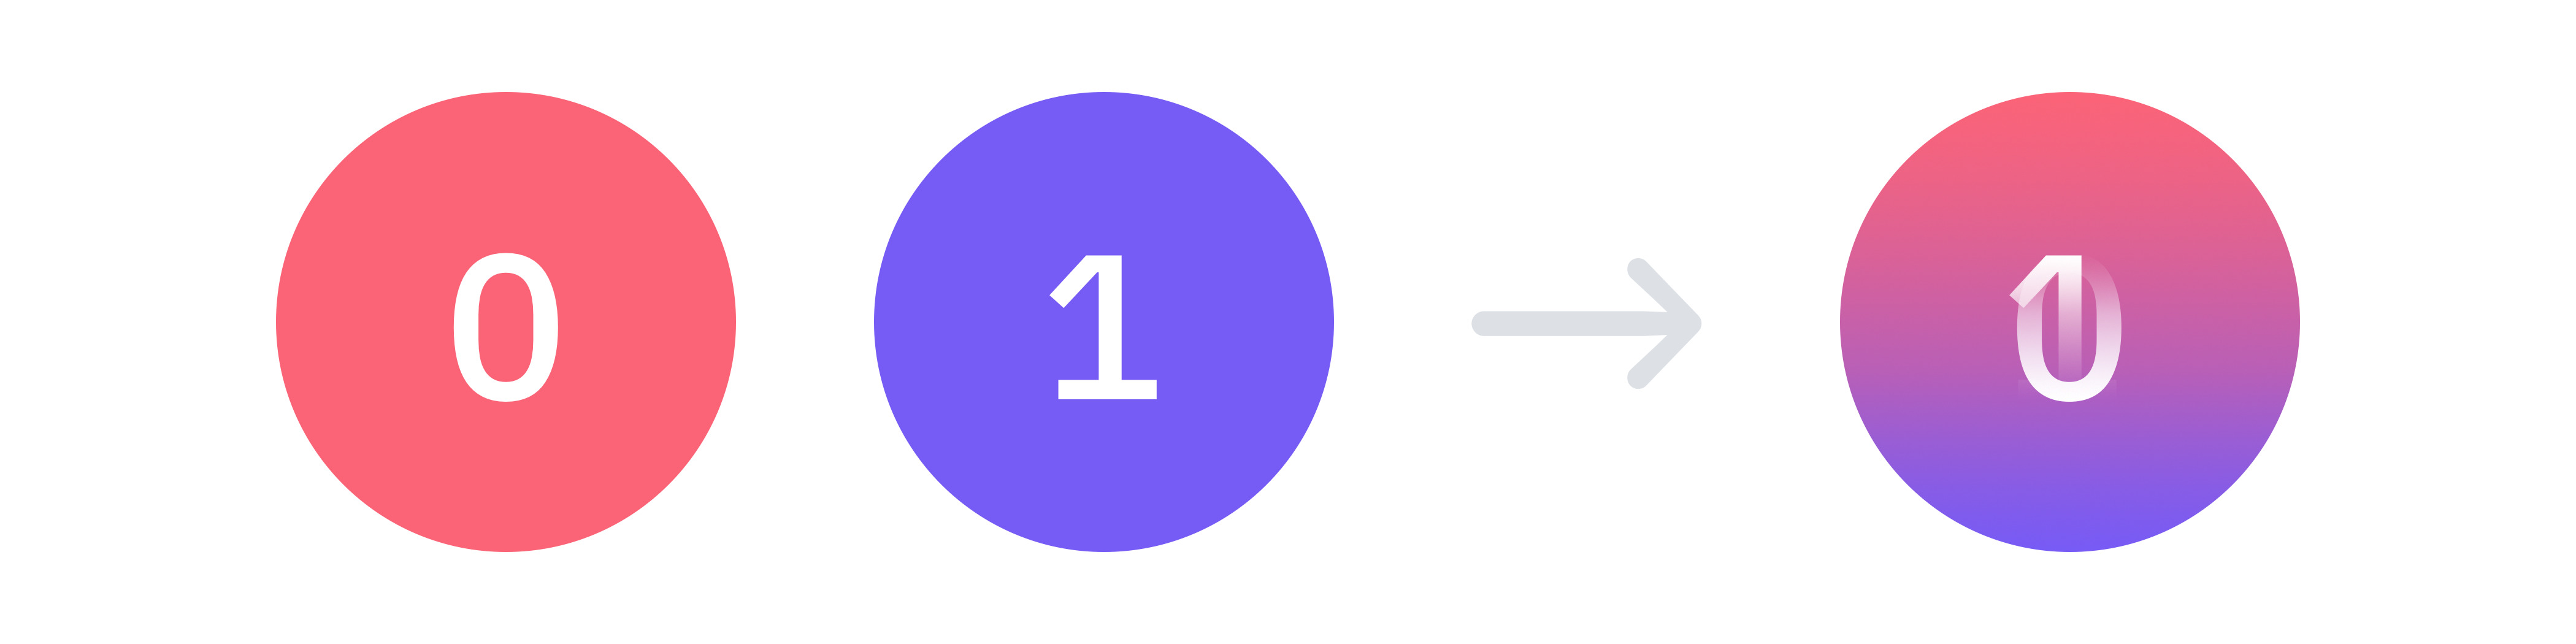
\includegraphics[alt={Testo alternativo dell'immagine}, width=1\columnwidth]{img/quantum_superposition.jpeg}
    \caption{Lorem}
    \label{fig:enter-label}
\end{figure}

\lipsum[1-2]

Lorem ipsum:
\begin{listing}[H]
\begin{minted}{python}
def recur_fibo(n):
   if n <= 1:
       return n
   else:
       return(recur_fibo(n-1) + recur_fibo(n-2))
nterms = 10
if nterms <= 0:
   print("Plese enter a positive integer")
else:
   print("Fibonacci sequence:")
   for i in range(nterms):
       print(recur_fibo(i))
\end{minted}
\caption{Fibonacci recursive}
\label{listing:py_fibo}
\end{listing}

\lipsum[1]

\newpage